\documentclass[12pt, twocolumn]{article}

\usepackage[T1]{fontenc}
\usepackage{lmodern}
\usepackage{microtype}
%\usepackage[notmath]{sansmathfonts}
%\usepackage{garamondx}
\usepackage{xcolor}
\usepackage{tikz}
\usepackage{classico}
\usepackage{gensymb} 
\usepackage{amsmath}
\usepackage{amssymb}
\usepackage{enumitem}
%\usepackage{FiraSans}
\usepackage[english]{babel}
\usepackage[pangram]{blindtext}
\usepackage{wrapfig}
\renewcommand\familydefault{\sfdefault}
%\renewcommand\sfdefault{phv}
%\normalfont
\usepackage[top=2.16in,left=0.65in,right=0.65in,bottom=0.73in]{geometry} 
 
\makeatletter
\def\parsecomma#1,#2\endparsecomma{\def\page@x{#1}\def\page@y{#2}}
\tikzdeclarecoordinatesystem{page}{
    \parsecomma#1\endparsecomma
    \pgfpointanchor{current page}{north east}
    % Save the upper right corner
    \pgf@xc=\pgf@x%
    \pgf@yc=\pgf@y%
    % save the lower left corner
    \pgfpointanchor{current page}{south west}
    \pgf@xb=\pgf@x%
    \pgf@yb=\pgf@y%
    % Transform to the correct placement
    \pgfmathparse{(\pgf@xc-\pgf@xb)/2.*\page@x+(\pgf@xc+\pgf@xb)/2.}
    \expandafter\pgf@x\expandafter=\pgfmathresult pt
    \pgfmathparse{(\pgf@yc-\pgf@yb)/2.*\page@y+(\pgf@yc+\pgf@yb)/2.}
    \expandafter\pgf@y\expandafter=\pgfmathresult pt
}
\makeatother

\newcommand{\specialcell}[2][c]{%
  \begin{tabular}[#1]{@{}l@{}}#2\end{tabular}}
\newcommand{\specialcellr}[2][r]{%
  \begin{tabular}[#1]{@{}r@{}}#2\end{tabular}}
%\addtolength{\skip\footins}{0pc plus 2pt}
\usepackage{titlesec}

\titlespacing*{\subsection}
{0pt}{0ex plus 0.2ex minus .2ex}{0.5ex plus .2ex}

\usepackage{booktabs}
\usepackage{lipsum}
\def\labelitemi{--}

\begin{document}
\thispagestyle{empty}\sffamily

\noindent ValBal\footnote{\sffamily The name is a contraction of ``Valve'' and ``Ballast''} is a high altitude latex balloon platform that controls its altitude by venting lifting gas and dropping ballast mass. This extends the life of a low-cost latex balloon from a few hours to a record-breaking 5 days. It's designed to facilitate a broad range of high altitude research thanks to its unique ability to maintain and dynamically transition between altitudes.

\begin{tikzpicture}[remember picture,overlay]
\fill[fill={rgb:red,190;green,30;blue,45}] (page cs:-1,1) rectangle (page cs:1,0.7);
\node (myfirstpic) at (page cs:-0.7,0.85) {
\includegraphics[height=0.15\textheight]{ssilogo.png}};
\node[color=white,anchor=west] (datasheet) at (page cs:-0.47,0.935) {\sffamily\fontsize{16}{20}\selectfont \textsc{Stanford Student Space Initiative}};
\node[color=white,anchor=west] (datasheet) at (page cs:-0.47,0.85) {\sffamily\fontsize{35}{40}\selectfont ValBal};
\node[color=white,anchor=west] (datasheet) at (page cs:-0.47,0.76) {\sffamily\fontsize{16}{20}\selectfont Altitude controlled latex high altitude balloon system};
\end{tikzpicture}
%\textbf{ValBal} is a high-altitude balloon platform that 
%\vspace{-.4cm}
%\subsection*{\sffamily Highlights}
%\vspace{1ex}
\vspace{0.15cm}

\def\power#1#2#3{\emph{Above $-$#1 \textdegree C:} #2~#3}
\begin{center}
\begin{tabular}{rl}
\toprule
\textbf{Altitude range} & \specialcell[t]{\emph{Standard:} 12.25--17 km\\\emph{Extended:} 0--23 km}\\\midrule
%\textbf{Peak power} & \specialcell[t]{\power{10}{3}{W}\\\power{40}{500}{mW}\\\power{60}{100}{mW}\\\power{70}{---}{}}\\\midrule
%\specialcellr[t]{\textbf{Cumulative}\\\textbf{energy}} & \specialcell[t]{\emph{24~hours:} 68~Wh\\\emph{48~hours:} 56~Wh\\\emph{72~hours:} 44~Wh}\\\midrule
\textbf{Endurance\footnotemark} & \specialcell[t]{\emph{No payload:} 5~days\\\emph{1~kg payload:} 3~days\\\emph{5~kg payload:} 1~day}\\\midrule
\textbf{Communications} & \specialcell[t]{  \begin{minipage}[t]{0.5\linewidth}
\item Iridium, 8\textcent/50 byte.
\item Custom 433~MHz radio, ~5~kBps line-of-sight.
\end{minipage}\vspace{1mm} }\\\midrule
\textbf{Cost\footnotemark} & \specialcell[t]{\emph{Consumables:} \$400\\\emph{Reusables:} \$1000}

%\\\midrule    \multicolumn{2}{c}{\footnotesize\begin{minipage}[t]{0.9\linewidth}\textbf{\small Notes:}
%\begin{itemize}[parsep=1ex,itemsep=-1ex]
%\item Many of the design parameters are flexible, and can be customized on a per mission basis.
%\item In particular, energy can be easily increased at a density of 300~Wh/kg, at the cost of payload; similarly for peak power.%; peak power at 
%\item An endurance of five days was demonstrated with zero payload. This reflects our current best mission, but we believe that longer missions are feasible with the system.
%\end{itemize}\end{minipage}\vspace{1mm}}
\\\bottomrule
\end{tabular}
\footnotetext[2]{\sffamily This reflects our current best mission, but we believe that longer missions are feasible with the system.}
\end{center}
{\footnotesize  
\vspace{0.4cm}
\begin{center}
\noindent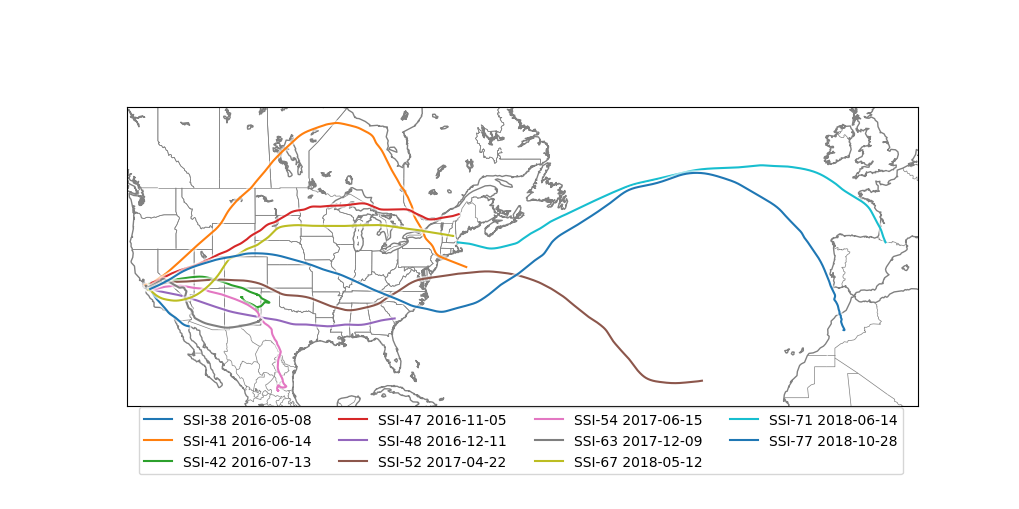
\includegraphics[width=\linewidth,trim={2.9cm 1.3cm 2cm 1.5cm},clip]{allflights.png}
\end{center}
\vspace{-.5cm} 
\paragraph{\sffamily Flight heritage:} The system has been developed though more than 20 test flights, 10 of which are shown above.%\vspace{-.4cm} 
%\section*{\sffamily Highlights}

%\begin{minipage}{\linewidth}
\vspace*{\fill}
\begin{center}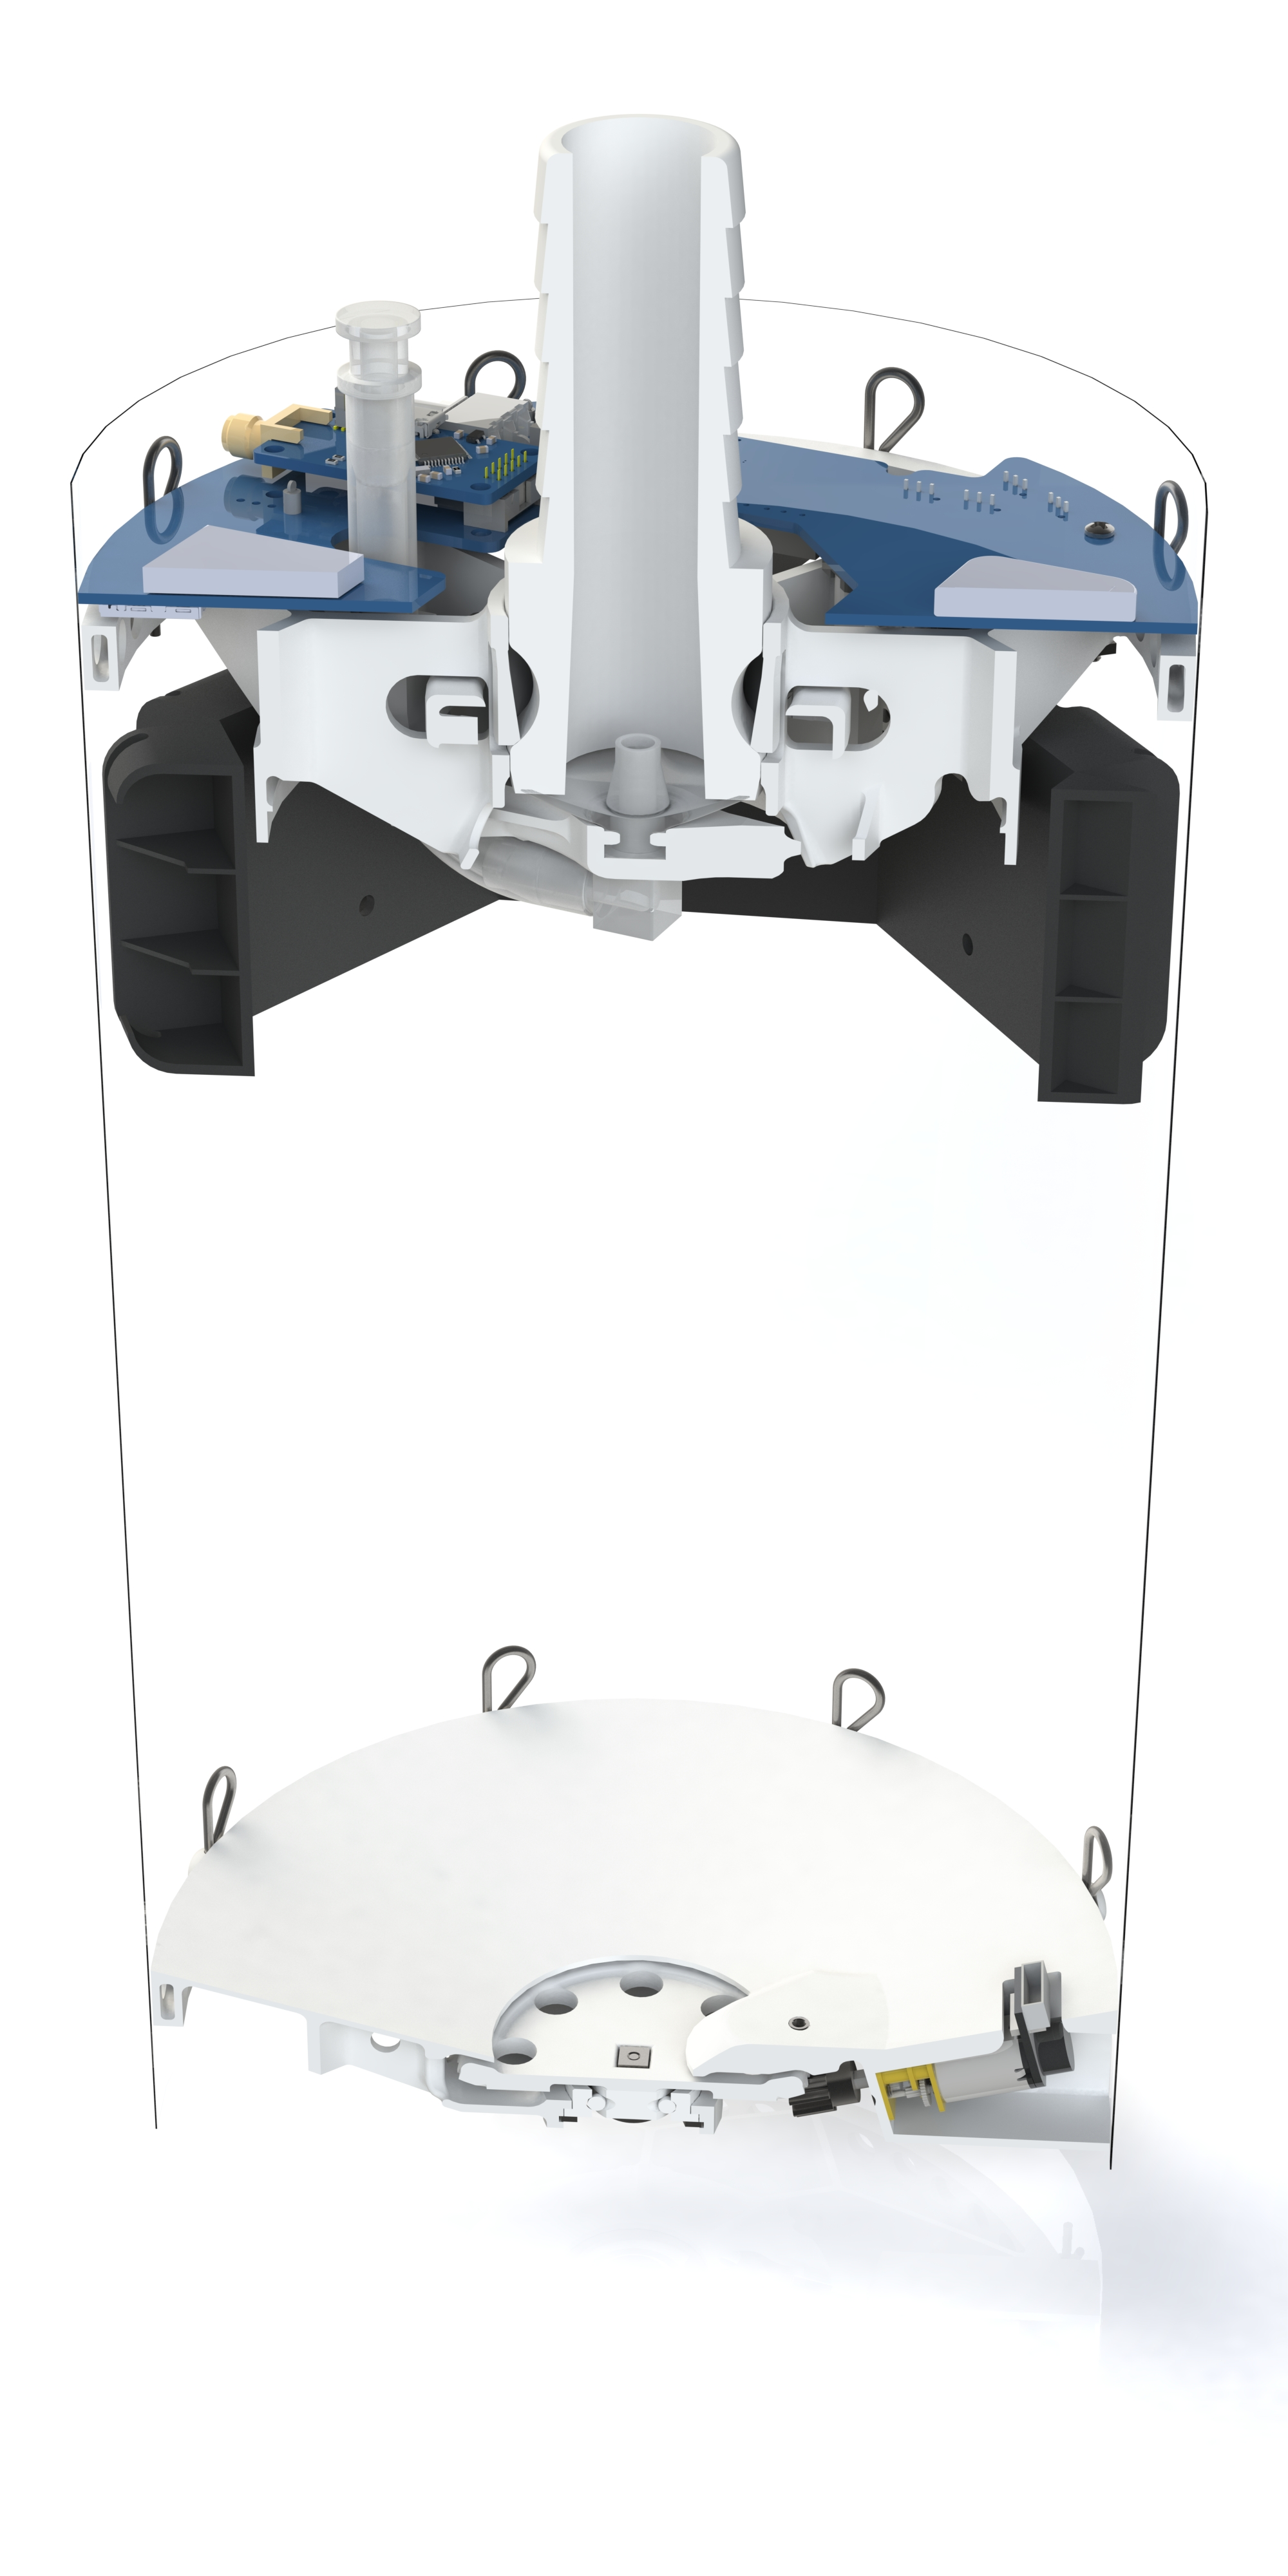
\includegraphics[width=0.5\linewidth,trim={0cm 13cm 0cm 5cm},clip]{render.jpg}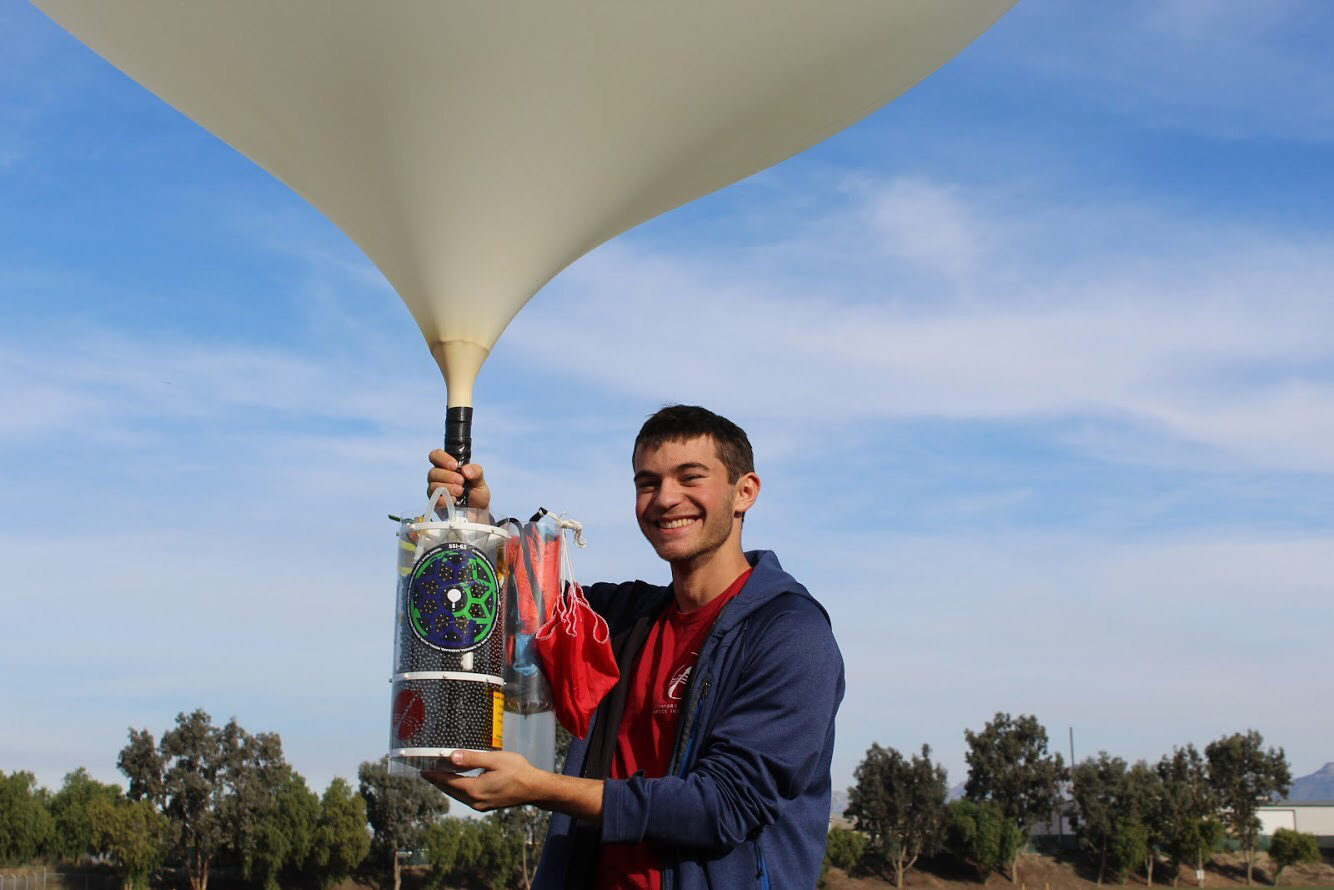
\includegraphics[width=0.5\linewidth,trim={12cm 2cm 25cm 12cm},clip]{vbpic.jpg}\end{center}
\paragraph{\sffamily Ease of assembly: } ValBal requires only six custom components and can be assembled in under 2 hours. No manual machining, cutting, gluing, or soldering is required.\footnotemark
\footnotetext[3]{\sffamily System can be reflown many times if recovered.}\footnotetext{\sffamily Above image shows a slightly older version than the current design.}

\vspace{0.41cm} 

\begin{center}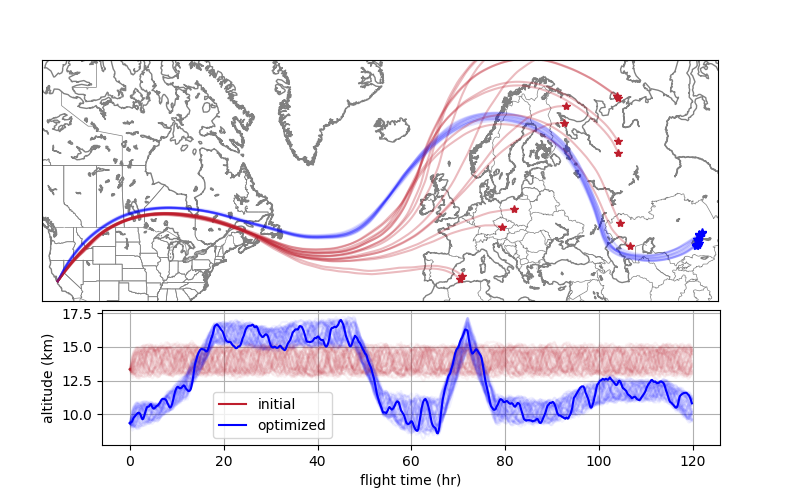
\includegraphics[width=\linewidth,trim={1cm 0.3cm 2cm 1.5cm},clip]{trajfig.png}\end{center}\vspace*{-0.6cm}
\paragraph{\sffamily Control capabilities:} Plot of possible 5-day flightpaths for a given launch time through monte carlo simulation with NOAA data. Red: altitude-bounded flight plans with no objective. Blue: flight plans optimized for distance.

%\end{minipage}
}


\end{document}